Cominciamo a discutere di qualche argomento di elettronica partendo dalla base, quindi partendo dai segnali che fuoriescono da un rivelatore e l'elettronica associata. Parleremo dei possibili segnali che fuoriescono dai rivelatori, che tipo di segnali possono fuoriuscire, come possono essere trattati, quindi che tipo di elettronica si può utilizzare e come possono essere anche trasportati da un modulo elettronico a un altro. 

\section{Rivelatori visuali}

%La prima domanda che ci faremo è se dai rivelatori sono sempre usciti dei segnali elettrici oppure quando è nata la fisica in realtà questo problema non c'era.

\subsection{Emulsioni nucleari}

I primi rivelatori che furono adoperati soprattutto nel campo della fisica nucleare, grazie ai quali furono effettuati diverse scoperte molto importanti, erano dei rivelatori visuali. Infatti i primi rivelatori erano basati sulla visualizzazione di tracce delle particelle in pellicole fotografiche o emulsioni nucleari, le quali potevano essere impressionate, potendo dunque mostrare il passaggio di particelle. Possiamo vedere un esempio nella seguente figura, raffigurante le tracce che si producono a seguito di un'interazione di uranio-238 con un energia di quasi un GeV per nucleone:
\begin{figure}[H]
   \centering
   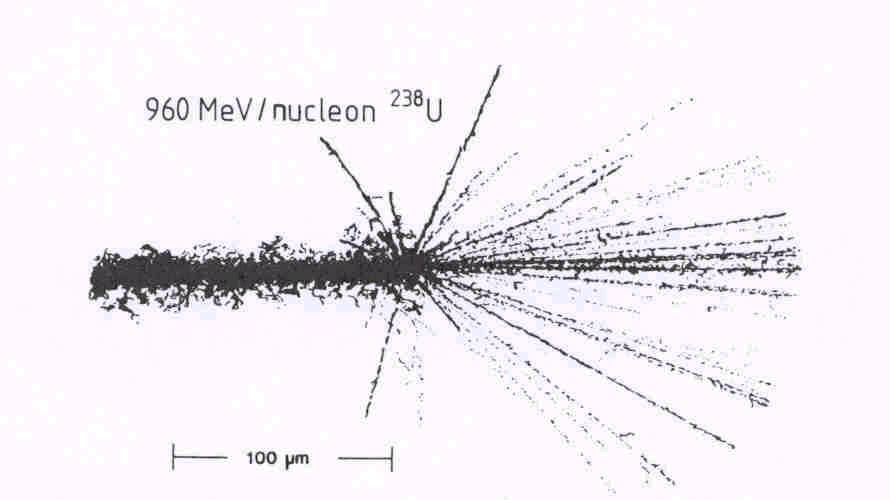
\includegraphics[width=0.6\textwidth]{immagini/emulsione_nucleare.png}
\end{figure}
Questo nucleo di uranio interagisce con un nucleo dell'emulsione nucleare, dando luogo a una serie di prodotti secondari. La traccia più spessa è quindi dovuta al passaggio dello ione pesante, mentre le tracce che vediamo subito dopo sono tutti i prodotti di questa interazione. Tutte queste sono delle tracce lineari.

Oltre all'informazione sul dove è passata la particella, non abbiamo molte altre informazioni aggiuntive, come ad esempio l'energia o il tipo di particella che dà luogo alla traccia. Sebbene quindi abbiamo l'enorme vantaggio di poter visualizzare il percorso di una particella, al tempo stesso è molto difficile l'interpretazione, cioè avere altre informazioni. Ad essere precisi, abbiamo un'altra informazione: notiamo che c'è un'enorme differenza tra la traccia in ingresso, quella dell'uranio 238, e le tracce prodotte successivamente all'interazione. Il motivo è che lo spessore della traccia dipende dal $\dv*{E}{x}$ della particella, per cui in generale le particelle cariche pesanti, che hanno un $\dv*{E}{x}$ considerevole, in un'emulsione nucleare producono una traccia che ha dimensioni più grandi, tant'è che come vediamo in figura l'$\rm ^{238}U$, che è uno ione pesante, deposita molta energia e di conseguenza la larghezza della traccia è notevole.

Se utilizzassimo un campo magnetico, le particelle cariche comincerebbero a seguire una traiettoria circolare, quindi in quel caso potremmo misurare l'impulso della particella, aumentando le informazioni che abbiamo a disposizione.

Che dimensioni hanno queste tracce? Ovviamente sono tracce molto piccole, dell'ordine di centinaia di micron, dunque devono essere analizzate al microscopio. Questi rivelatori, proprio per le dimensioni che si raggiungono, sono in assoluto i rivelatori che hanno la migliore risoluzione spaziale. Ad oggi però sono dei rivelatori che si utilizzano pochissimo, perché sono dei rivelatori passivi, quindi non hanno bisogno di un'elettronica. Sebbene ciò da un lato costituisca un vantaggio, dall'altro ci costringe a dover lasciare le emulsioni esposte alla radiazione e quando siamo soddisfatti di quello che abbiamo raccolto le dobbiamo prelevare, sviluppare, quindi trattare chimicamente e poi analizzare in maniera visiva attraverso un microscopio ottico, quindi c'è un tempo morto tra quando avviene l'esposizione e quando avviene l'analisi del dato, pertanto non abbiamo un dato in tempo reale.

Ad oggi sono utilizzate veramente poco, però ci sono degli esperimenti che ancora adoperano le emulsioni nucleari, ad esempio l'esperimento OPERA al Gran Sasso.

\subsection{Camere a nebbia}

\begin{minipage}{0.36\textwidth}
   \begin{figure}[H]
      \centering
      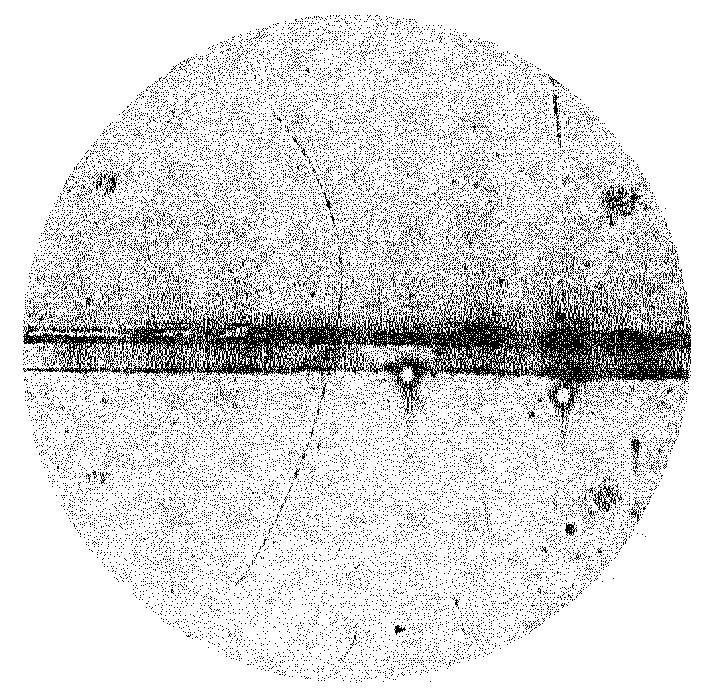
\includegraphics[width=0.7\textwidth]{immagini/camera_a_nebbia.png}
   \end{figure}
\end{minipage}
\begin{minipage}{0.63\textwidth}
   \vspace{0.7cm}Altri esempi di rivelatori che visualizzano le tracce sono le camere a nebbia, che sono dei rivelatori costituiti da camere dove all'interno si crea una condizione di vapore sovra-saturo, quindi una condizione abbastanza instabile, e al passaggio di una particella carica si vengono a creare delle goccioline di condensa lungo la traiettoria della particella.
\end{minipage}

\vspace{0.5cm}Anche in questo caso la dimensione della traccia cambia in base al tipo di particella, ad esempio per particelle cariche leggere vediamo dei percorsi molto sottili a zigzag perché queste interagiscono e cambiano traiettoria, mentre per particelle più pesanti come le $\alpha$ vediamo delle tracce corte e molto larghe.

Anche in questo caso se si accoppia l'apparato con un campo magnetico si può avere qualche informazione in più sulla traccia, però anche stavolta non abbiamo un segnale elettrico ma soltanto una visualizzazione, dunque al massimo possiamo scattare una foto.

\subsection{La camera a bolle}
Un altro esempio di rivelatore visuale è la camera a bolle, che è molto simile alla camera a nebbia però funziona con un liquido e il passaggio di una particella crea delle microbolle lungo il percorso che permettono di visualizzare la traccia.

\begin{figure}[H]
   \centering
   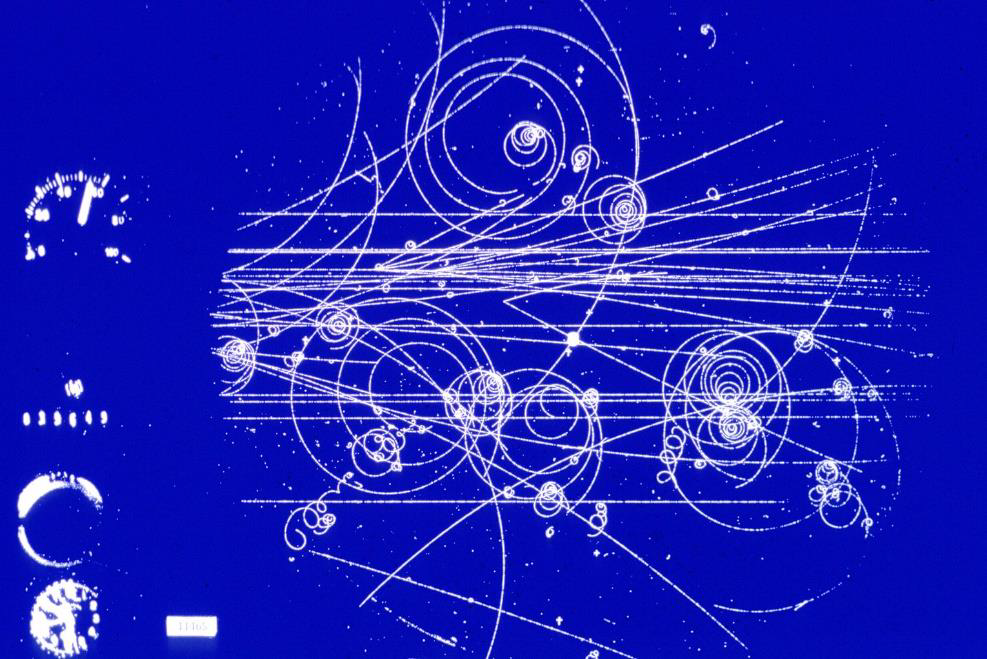
\includegraphics[width=0.6\textwidth]{immagini/camera_a_bolle.png}
\end{figure}

In figura possiamo vedere il percorso che seguirebbe una particella in un campo magnetico, che è una spirale perché man mano la particella perde energia e quindi via via il raggio si riduce.

All'inizio queste tracce si analizzavano a mano. Quello che si faceva era stampare queste fotografie e analizzarle manualmente, che è una procedura molto scomoda.

\section{Rivelatori moderni}

Ad oggi la maggior parte dei rivelatori produce in output un segnale elettrico che può essere di varia natura e che trasporta in sé svariate informazioni, ad esempio sul tipo di particella, sull'energia oppure sul tempo di arrivo.

%\E chiaro che trattare un segnale richiede un'opportuna elettronica. 

Quando parliamo di un segnale, normalmente intendiamo una variazione nel tempo di una tensione o di una corrente.

\begin{figure}[H]
   \centering
   \begin{tikzpicture}
      \draw[->] (0,0) -- (8,0) node[right] {$t$};
      \draw[->] (0,-4) -- (0,1) node[above] {$V$};
      \draw[thick,red] plot[smooth,domain=0:7.7] (\x, {-10*\x * exp(-\x)});
    \end{tikzpicture}
\end{figure}

Generalmente ragioniamo in termini di tensione, quindi su un grafico avente come asse temporale quello orizzontale e come asse delle tensioni quello verticale avere un segnale (impulsivo nel caso della figura) equivale a dire che la tensione dal valore 0 o dal valore di baseline diminuisce o aumenta (a seconda che si tratti di un segnale negativo o positivo) all'improvviso per poi ritornare alla baseline dopo un certo intervallo di tempo. Come abbiamo detto, questo segnale può trasportare diverse informazioni, quindi l'elettronica che si adopera a seguire deve essere pensata per estrarre da questo segnale le informazioni che ci servono. Abbiamo già visto un esempio di ciò utilizzando il fotomoltiplicatore in laboratorio: in quel caso sapevamo che l'informazione dal segnale che fuoriusciva dal fotomoltiplicatore che ci interessava era l'ampiezza ossia l'altezza di questo segnale, quindi tutti i moduli elettronici che si utilizzavano a seguire erano finalizzati alla misura dell'ampiezza del segnale, infatti c'era un amplificatore per aumentare l'ampiezza del segnale e un ADC che aveva lo scopo di misurare l'ampiezza e a tradurla in un numero da fornire al computer.

In generale, qualsiasi rivelatore (anche il più semplice) deve prevedere almeno un cavo attraverso cui deve viaggiare non solo la tensione ma anche il segnale che fuoriesce quando viene misurato il passaggio di una particella. Il caso in cui abbiamo un solo cavo è il caso banale, ma in esperimenti complessi, con più canali, bisogna gestire più segnali, dunque servono più cavi\footnote{Per avere un'idea di quanti cavi ci sono e della lunghezza di questi ci basta pensare che in un grosso esperimento a LHC la lunghezza totale dei cavi può essere anche di 3.000 km!}. Ci basta pensare alla camera a fili, in cui da ogni filo esce un segnale.

In ultima analisi, la realizzazione del cablaggio\footnote{Il cablaggio si riferisce all'insieme di fili e cavi utilizzati per collegare vari dispositivi o sistemi elettrici ed elettronici, permettendo il passaggio di energia o segnali.} è un'operazione che può durare anche diverso tempo. A complicare la situazione, si aggiunge il fatto che spesso si cerca di far passare i cavi in appositi passaggi sia per evitare di introdurre del material budget indesiderato nell'esperimento sia perché lo spazio a disposizione non è tutto quello che vogliamo, anche perché in grossi esperimenti spesso si hanno tanti rivelatori diversi a cui lavorano gruppi diversi, per cui è chiaro che bisogna condividere gli spazi. Per tutti questi motivi, il passaggio dei cavi è un'operazione che viene necessariamente studiata all'inizio di un esperimento.

\subsection{Trapsorto dei segnali}

Cosa viene trasportato in questi cavi?

\begin{itemize}[leftmargin=0.5cm]
   \item Alimentazioni per i rivelatori, i quali normalmente devono essere alimentati o con basse tensioni o con alte tensioni, come nel caso del fotomoltiplicatore il quale deve essere alimentato a 600 V, infatti nell'esperienza di laboratorio avevamo il modulo di alimentazione e un cavo che collegava questo fino al fotomoltiplicatore;
   \item Segnali di diversa natura;
   \item Segnali di controllo per le apparecchiature.
\end{itemize}

\vfill

\section{Segnali impulsivi}
Per prima cosa andiamo a vedere che tipo di segnali possono viaggiare in questi cavi.

Come abbiamo detto, per estrarre l'informazione racchiusa in questi segnali è necessario che siano processati con un opportuno sistema elettronico, allo scopo ad esempio di
\begin{itemize}[leftmargin=0.5cm]
   \item distinguere segnali di tipo differente;
   \item estrarre un'informazione sull'energia;
   \item estrarre un'informazione temporale.
\end{itemize}
e ovviamente lo scopo dipende dalla specifica applicazione del rivelatore.

Tipicamente, piuttosto che con segnali periodici, abbiamo a che fare con segnali impulsivi rappresentanti singoli eventi e le informazioni che vogliamo estrarre sono legate alle caratteristiche di questo segnale quali ad esempio l'ampiezza, la durata, la forma del segnale, la polarità, il tempo a cui arriva il segnale e che dipendono dalla misura che stiamo effettuando.

\subsection{Terminologia}
Diamo alcune terminologie importanti quando si parla di segnali. Consideriamo il segnale mostrato in figura, dove è riportato il tempo in ascisse e la tensione in ordinate:

\begin{figure}[H]
   \centering
   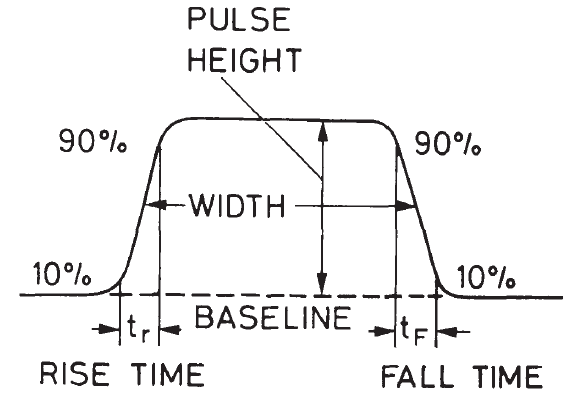
\includegraphics[width=0.5\textwidth]{immagini/terminologia_segnali_1.png}
\end{figure}

Questo segnale parte da un valore costante, aumenta, si stabilizza e poi dopo un po' diminuisce per ritornare al valore iniziale. Si tratta quindi di impulso con una forma un po' più squadrata rispetto a quelle che abbiamo visto in precedenza, ma ci torna utile per dare delle definizioni. Per un segnale, possiamo definire:

\begin{itemize}[leftmargin=0.5cm]
   \item l'\textit{altezza} o \textit{ampiezza} (in inglese pulse height), ossia la distanza tra la baseline e il valore massimo che viene raggiunto dal segnale. In essa potrebbe essere racchiusa ad esempio l'informazione sull'energia depositata nel rivelatore;
   \item la \textit{durata} del segnale, ossia la larghezza (in inglese pulse width),che vediamo rappresentata in orizzontale.
   \item il \textit{tempo di salita} o il \textit{tempo di discesa} (rispettivamente rise time e fall time in inglese), che vengono definiti andando a vedere il tempo necessario perché il segnale passi dal 10\% al 90\% della sua massima ampiezza nel caso del rise time o viceversa dal 90\% al 10\% nel caso del fall time.
\end{itemize}

Il segnale appena visto è un segnale ideale. In realtà si possono presentare dei segnali un po più particolari, con delle deformazioni del segnale, come nella seguente figura:
\begin{figure}[H]
   \centering
   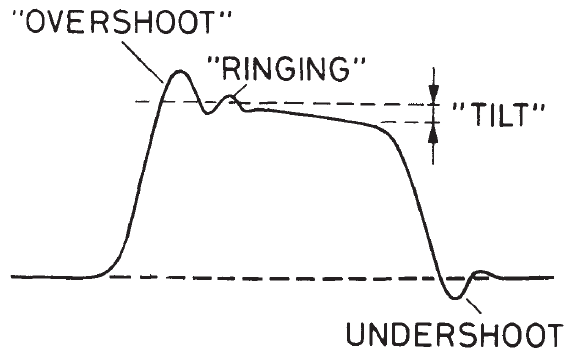
\includegraphics[width=0.5\textwidth]{immagini/terminologia_segnali_2.png}
\end{figure}
Come deformazioni potremmo avere:
\begin{itemize}[leftmargin=0.5cm]
   \item casi in cui il segnale va oltre il valore massimo (detto overshoot);
   \item casi in cui il segnale va al di sotto della baseline (detto undershoot);
   \item effetti di ringing, cioè delle oscillazioni del segnale attorno a un valore;
   \item effetti di tilt, cioè un segnale che dovrebbe essere piatto in realtà man mano presenta una leggera diminuzione della sua ampiezza.
\end{itemize}
Tutti questi sono degli effetti che non vorremmo ma che inevitabilmente, quando il segnale viene trasportato o viene gestito da apparati elettronici, si potrebbero presentare.

\vspace{0.2cm}I segnali potrebbero inoltre essere unipolari o bipolari. Si definiscono unipolari quando presentano un solo lobo, bipolari quando attraversano la baseline.
\begin{figure}[H]
   \centering
   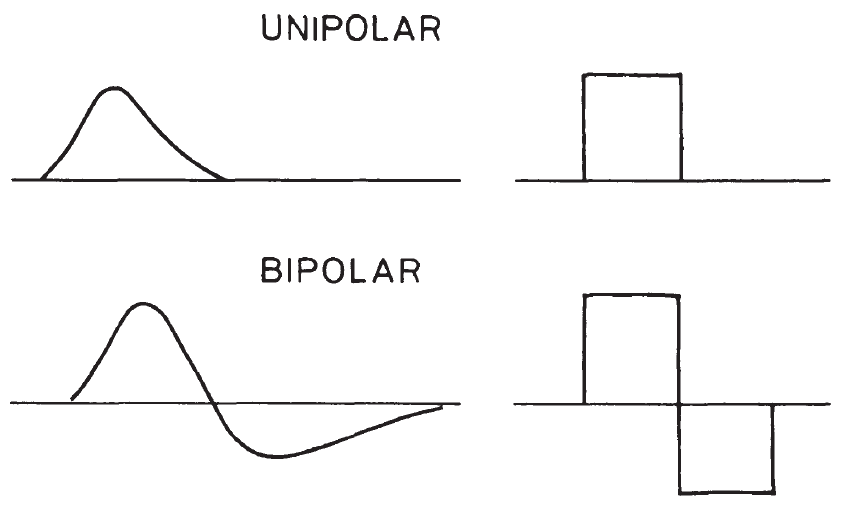
\includegraphics[width=0.6\textwidth]{immagini/segnali_unipolari_e_bipolari.png}
\end{figure}
Nella figura possiamo vedere un esempio di segnale unipolare e uno di segnale bipolare sia nel caso di un segnale analogico che nel caso di un segnale logico, differenza che spiegheremo a breve.

\vspace{0.2cm}Un'ulteriore distinzione molto importante è quella tra segnali analogici e segnali logici. Nel segnale analogico l'informazione è codificata in modo continuo in una caratteristica del segnale (ad esempio l'ampiezza o la forma) ed è proporzionale al valore dell'informazione. Tornando alla figura precedente, i segnali che vediamo alla sinistra sono esempi di segnali analogici, il cui valore di tensione varia in modo continuo nel tempo. Viceversa, il segnale è logico\footnote{A volte si parla di segnale digitale anziché logico, ma in realtà è più corretto dire segnale logico.} quando può assumere dei valori discreti, dunque la tensione che andiamo a visualizzare all'oscilloscopio non può assumere qualsiasi valore, ma soltanto dei valori discreti. Tipicamente ci sono in totale due valori discreti, perché sono associati allo stato 0 e allo stato 1, e a seconda dello standard ad essi viene associato un certo livello di tensione. \E chiaro che l'informazione che viene trasportata in questo tipo di segnale è inferiore rispetto a quello del segnale analogico, tuttavia essi sono più affidabili poiché è più difficile che l'informazione sia deteriorata nel corso del
trasporto.

Un'altra distinzione che possiamo fare è quella tra segnali lenti e segnali veloci. Questo aspetto si valuta andando a guardare il fronte di salita di un segnale, cioè il tempo che impiega il segnale per passare dal 10\% al 90\% della sua ampiezza. In particolare i segnali si definiscono
\begin{itemize}
   \item veloci quando hanno tempi di salita di alcuni nanosecondi o meno;
   \item lenti quando hanno tempi di salita di centinaia di nanosecondi o anche microsecondi.
\end{itemize}

%Guardiamo adesso qualche tipico esempio di segnale:

\begin{esempio}[Esempio di segnale veloce]
   In figura possiamo vedere la rappresentazione all'oscilloscopio di un tipico segnale veloce:
   \begin{figure}[H]
      \centering
      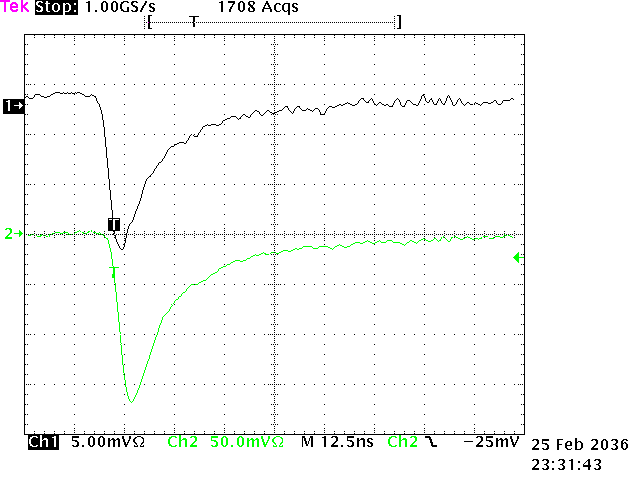
\includegraphics[width=0.6\textwidth]{immagini/esempio_segnale_veloce.png}
   \end{figure}
   Ricordiamo che, in un'oscilloscopio, sull'asse orizzontale si rappresenta il tempo e sull'asse verticale la tensione. Inoltre c'è la possibilità di cambiare sia la scala dei tempi che quella della tensione in base al segnale che vogliamo visualizzare. In questo caso la scala dei tempi (cioè ogni quadrettino) corrisponde a 12.5 ns, mentre la scala verticale corrisponde a 5 mV.
   
   Concentrandoci sul segnale, notiamo che il tempo di salita\footnotemark, cioè il tempo in cui il segnale passa dal 10\% al 90\% del suo valore massimo, ha una durata molto piccola, dell'ordine del nanosecondo, per cui siamo nel caso di segnali veloci.
\end{esempio}

\footnotetext{Anche se il segnale sta scendendo si chiama comunque tempo di salita.}

\begin{esempio}[Esempio di segnale lento]
   Nella seguente figura possiamo invece vedere un tipico esempio di segnale lento:
   \begin{figure}[H]
      \centering
      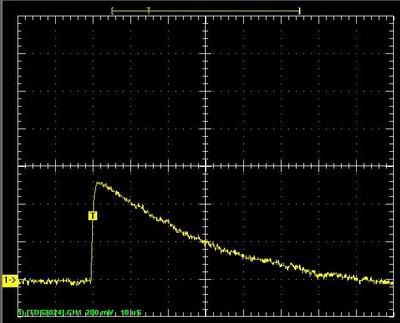
\includegraphics[width=0.6\textwidth]{immagini/esempio_segnale_lento.png}
   \end{figure}
   Notiamo che la scala dei tempi è molto diversa rispetto al caso precedente, infatti stavolta ogni quadretto equivale a $10 \; \rm \mu s$, per cui se ingrandissimo la zona del fronte di salita\footnotemark\, ci renderemo conto che esso si esaurisce in tempi dell'ordine di centinaia di nanosecondi o anche un microsecondo, quindi siamo nel caso di segnali lenti.
\end{esempio}

\footnotetext{Il fronte di salita è la porzione del segnale in cui avviene la variazione da un livello inferiore a un livello superiore. In pratica, è la fase in cui il segnale inizia a crescere da uno stato basso a uno stato alto.}

I segnali veloci si usano quando siamo interessati all'informazione di timing. Supponiamo ad esempio di voler misurare il tempo di volo di un raggio cosmico nel passare da un rivelatore ad un altro posto alla distanza di 1 metro dal primo: poiché queste particelle viaggiano a velocità prossime a quella della luce nel vuoto, su una base di volo di un metro ci aspettiamo un tempo di volo di $3-4 \; \rm ns$, quindi un segnale lento risulterebe inutile per questa applicazione di timing.

I segnali lenti si utilizzano invece soprattutto in spettroscopia, perché in quel caso non siamo interessati al timing, bensì all'affidabilità sull'informazione legata ad esempio all'ampiezza perché vogliamo misurare l'energia di una particella.

\subsection{Banda passante}
I segnali veloci sono difficili da trattare perché, come vedremo, ogni modulo elettronico presenta una banda passante, e questa ha conseguenze importanti sul segnale che stiamo gestendo.

Per parlare di banda passante dobbiamo immaginare il segnale non più nel dominio del tempo come abbiamo fatto fino ad adesso\footnote{Infatti finora abbiamo studiato i segnali andando a guardare la loro evoluzione nel tempo.}, bensì nel dominio delle frequenze. Per fare ciò utilizziamo la trasformata di Fourier, la quale ci dice che un qualunque segnale (anche aperiodico) rappresentato dalla funzione $f(t)$ può essere decomposto in una sovrapposizione di segnali sinusoidali puri di ampiezza infinitesima:
\begin{equation*}
   f(t)=\frac{1}{\sqrt{2\pi}} \int_{-\infty}^{+\infty} g(\omega) e^{i \omega t} \dd{\omega}
\end{equation*}
dove $g(\omega)$ è la trasformata di Fourier. Invertendo tale relazione si ottiene
\begin{equation*}
   g(\omega)=\frac{1}{\sqrt{2\pi}} \int_{-\infty}^{+\infty} f(t) e^{-i \omega t} \dd{t}
\end{equation*}

Notiamo che l'integrale in $\dd{\omega}$ si estende da $-\infty$ a $+\infty$, il che significa che tutte le frequenze giocano un ruolo nella modellazione della funzione $f(t)$. Pertanto, affinché un dispositivo elettronico possa trattare fedelmente le informazioni contenute in questo segnale, esso deve essere in grado di rispondere uniformemente a un intervallo infinito di frequenze. Ovviamente, in un circuito reale, questo è impossibile: saranno sempre presenti componenti resistivi e reattivi che filtreranno alcune frequenze più di altre, limitando così la risposta a un intervallo finito di frequenze.

La banda passante di un apparato elettronico rappresenta sostanzialmente l'intervallo di frequenze delimitato dai punti in cui la risposta scende a $-3$ dB. Per comprendere meglio tale concetto facciamo un esempio: immaginiamo di voler adoperare un amplificatore per ascoltare della musica e di averne fissato il guadagno (o come viene detto in gergo di averne fissato il volume) tramite l'opportuna manopola. Idealmente vorremmo che questo amplificatore funzioni allo stesso modo indipendentemente dalla frequenza del suono che stiamo inviando ad esso, ma non è detto che sia così. Infatti potremmo stare lavorando con un amplificatore di scarsa qualità, per cui la risposta cambia in base alla frequenza.

Possiamo vedere un esempio di risposta di un apparato in funzione della frequenza del segnale che stiamo inviando nella seguente figura, dove si rappresenta la frequenza in ascisse e la risposta relativa in ordinate:

\begin{minipage}{0.45\textwidth}
   \begin{figure}[H]
      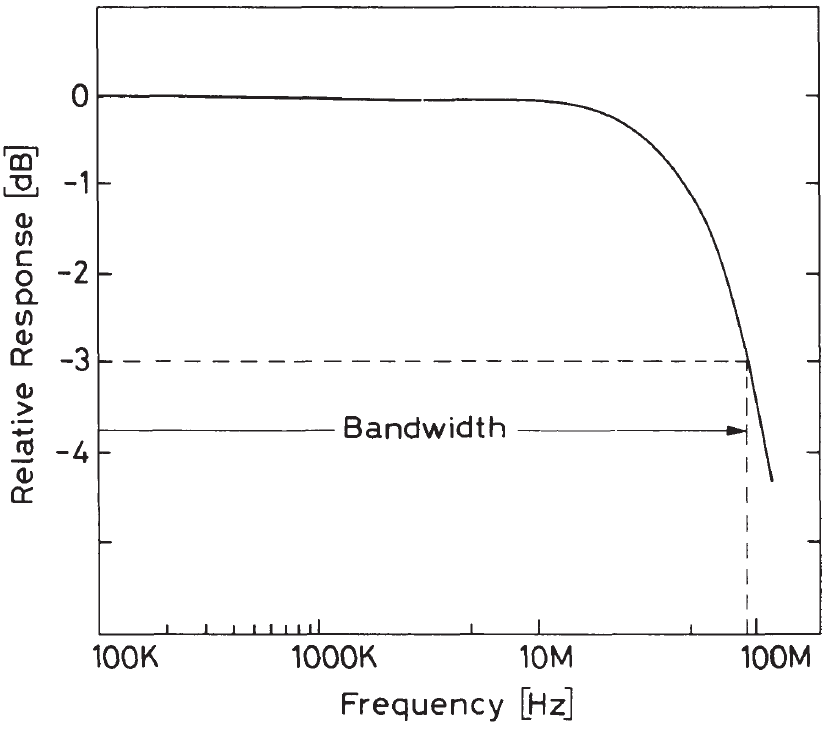
\includegraphics[width=0.99\textwidth]{immagini/banda_passante.png}
   \end{figure}
\end{minipage}
\begin{minipage}{0.54\textwidth}
   Quello che si vede è sostanzialmente una risposta costante, piatta per un certo intervallo di frequenze e poi all'improvviso la risposta dell'apparato elettronico diminuisce. L'intervallo della banda passante è indicato dal punto in cui si raggiunge il limite dei $-3 \; \rm dB$. Se ad esempio riconsideriamo l'esempio dell'amplificatore che utilizziamo per ascoltare la musica, se questo avesse una banda passante a 10 kHz,\footnotemark\, allora tutti i suoni da 10 kHz a 20 kHz non verrebbero riprodotti bene.
\end{minipage}

\footnotetext{Ovviamente non esistono amplificatori per il suono di questo tipo, perché il suono udibile all'orecchio umano arriva almeno a 20 kHz, quindi bisogna certamente superare questa soglia per poter gestire in maniera corretta i suoni.}

Precisiamo che tale limite è imposto per definizione, cioè siamo noi che scegliamo di dire che l'apparato funziona abbastanza bene in tale intervallo di frequenze e che nel momento in cui usciamo fuori da questo intervallo l'apparato non sta rispondendo bene, in quanto c'è un'attenuazione che è più grande di 3 dB.

Vediamo perché si sceglie proprio questa soglia. Ricordiamo che un deciBel è un decimo di Bel ed è definito come segue
\begin{equation*}
   1 \text{ dB}
   =10 \log_{10} \qty( \frac{V_1}{V_2} )
\end{equation*}
dove $V_1$ è la tensione in entrata e $V_2$ quella in uscita.
Vediamo a cosa corrisponde, secondo questa definizione, il valore di 3 dB: sostituendo si ha
\begin{equation*}
   10 \log_{10} \qty( \frac{V_1}{V_2} )=3
   \implies
   \log_{10} \qty( \frac{V_1}{V_2} )=0.3
   \implies
   \frac{V_1}{V_2}=10^{0.3}=1.995 \approx 2
\end{equation*}
Il risultato trovato ci dice che il segnale in uscita si è sostanzialmente dimezzato (cioè è stato attenuato della metà) rispetto a quello in entrata.

In sintesi, definire la banda passante di un modulo elettronico equivale a dare l'indicazione sull'intervallo di frequenze entro cui un apparato di questo tipo funziona correttamente, quindi il segnale viene riprodotto bene. Se ritorniamo alla rappresentazione del segnale mediante trasformata di Fourier, la banda passante rappresenta l'intervallo di integrazione della trasformata. Vediamo allora, nel caso di un segnale impulsivo, come questo venga modificato a seconda dell'ampiezza della banda passante. Osserviamo la seguente figura, in cui è rappresentato un segnale impulsivo di tipo logico a cui di volta in volta è sovrapposta la trasformata di Fourier (indicata dalla linea tratteggiata) ottenuta per diverse ampiezze della banda passante:
\begin{figure}[H]
   \centering
   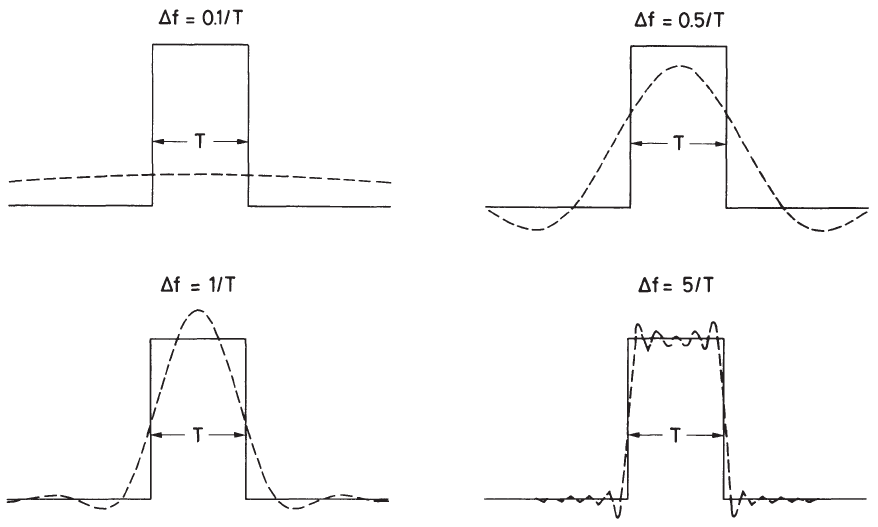
\includegraphics[width=0.8\textwidth]{immagini/banda_passante_segnale_impulsivo.png}
\end{figure}
Detta $T$ la durata del segnale, andiamo a studiare i casi in cui la banda passante ha ampiezza $\Delta f$ pari a multipli di $1/T$:
\begin{itemize}[leftmargin=0.5cm]
   \item Se $\Delta f=0.1/T$, che nel caso in cui $T=1 \; \rm \mu s$ equivale a 100 kHz, il segnale risulta completamente deformato, apparendo quasi piatto;
   \item Se $\Delta f=0.5/T$, che nel caso in cui $T=1 \; \rm \mu s$ equivale a 500 kHz, si vede una sorta di impulso, ma la forma è completamente diversa da quella squadrata che avevamo mandato in ingresso;
   \item Se $\Delta f=1/T$, che nel caso in cui $T=1 \; \rm \mu s$ equivale a 1 MHz, viene riprodotta meglio la baseline rispetto al caso precedente, ma il segnale, di per sé squadrato, viene ancora deformato di molto;
   \item Se arriviamo ad un intervallo $\Delta f=5/T$, che nel caso in cui $T=1 \; \rm \mu s$ equivale a 5 MHz, riusciamo finalmente ad avere una forma più realistica del segnale.
\end{itemize}
Da questo esempio capiamo che l'effetto della banda passante al variare della sua ampiezza è quello di rappresentare il segnale in maniera più o meno realistica, potendo deformare il segnale se scelta in maniera non opportuna. In particolare, possiamo dire che la minima banda passante $\Delta f$ per qualsiasi apparato elettronico per rappresentare in maniera ragionevole l'impulso deve essere almeno superiore a $1/T$, per cui ad esempio per trattare impulsi da 5 ns servono bande passanti di almeno 200 MHz.

Nel caso dell'elettronica nucleare, tipicamente tutti i moduli elettronici hanno bande passanti di almeno 500 MHz. Sebbene non sia banale avere queste bande passanti, ad oggi si sono raggiunti anche limiti più alti, arrivando anche a 1 GHz o 2 GHz in alcuni casi, per cui sono degli apparati ad alta fedeltà, che riproducono in maniera fedele il segnale di ingresso.

\subsection{Da segnali analogici a segnali logici}
Se abbiamo a che fare con un segnale analogico e vogliamo passare a un segnale logico, è necessario utilizzare un modulo elettronico\footnote{Nel seguito vedremo alcuni esempi di moduli elettronici, ma in questo corso non entreremo nel dettaglio del funzionamento di questi moduli, quindi come viene effettuata quell'operazione. Li vedremo come schemi a blocchi, quindi ci interessa sapere, rappresentandoli come dei blocchi, che tipo di segnale entra in ingresso, che tipo di segnale fuoriesce e qual è la funzione di questo modulo elettronico.} che prende il nome di \textit{discriminatore}, il quale ha la funzione di discriminare e dare luogo, partendo da un segnale analogico, ad un segnale logico in uscita. Schematicamente può essere rappresentato nel seguente modo:
\begin{figure}[H]
   \centering
   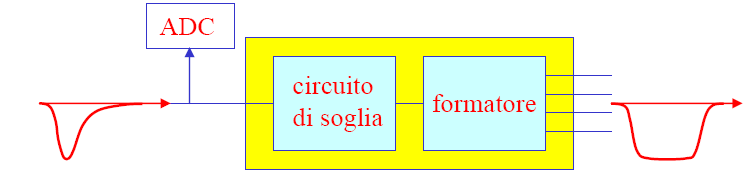
\includegraphics[width=0.8\textwidth]{immagini/discriminatore.png}
\end{figure}
In ingresso abbiamo un tipico segnale analogico, con un valore di tensione che varia in modo continuo nel tempo, e in uscita invece ci ritroviamo un segnale logico che può presentare solamente due valori possibili, o la baseline o un valore massimo.

All'interno, un discriminatore deve avere due componenti:
\begin{itemize}[leftmargin=0.5cm]
   \item Un circuito di soglia, cioè un circuito che va a confrontare l'ampiezza del segnale in ingresso con una soglia che stabilisce l'utente per decidere se l'altezza del segnale è superiore o no al valore minimo (la soglia) indicato dall'utente;
   \item Un formatore, che ha lo scopo di creare in uscita un segnale con un'opportuna forma.
\end{itemize}

Prima di parlare del discriminatore, vediamo gli standard che si usano. Infatti abbiamo detto che un segnale logico è un segnale che varia tra due valori, un valore che rappresenta lo zero logico e uno che rappresenta l'uno logico, ma non abbiamo detto a cosa corrispondano questi in termini di tensione. In altre parole, se mandiamo un segnale logico all'oscilloscopio, che livelli di tensione ci aspettiamo di trovare? La risposta è che dipende dallo standard che si utilizza.
\begin{figure}[H]
   \centering
   \begin{tikzpicture}
      \draw[very thick] (0,0) -- (1.5,0) -- (1.5,2) -- (3,2);
      \node[left=0.2cm] at (0,0) {$0$};
      \node[right=0.2cm] at (3,0) {0 V};
      \node[left=0.2cm] at (0,2) {$1$};
      \node[right=0.2cm] at (3,2) {$2 - 5$ V};
      \node[right=0.2cm] at (3,3) {TTL};
      \begin{scope}[shift={(7cm, 0cm)}]
         \draw[very thick] (0,2) -- (1.5,2) -- (1.5,0) -- (3,0);
         \node[left=0.2cm] at (0,2) {$0$};
         \node[right=0.2cm] at (3,2) {$-0.90$ V};
         \node[right=0.2cm] at (5,2) {0 V};
         \node[left=0.2cm] at (0,0) {$1$};
         \node[right=0.2cm] at (3,0) {$-0.80$ V};
         \node[right=0.2cm] at (5,0) {$-1.75$ V};
         \node[right=0.2cm] at (3,3) {NIM};
         \node[right=0.2cm] at (5,3) {ECL};
      \end{scope}
   \end{tikzpicture}
\end{figure}

Uno standard molto diffuso è il cosiddetto TTL, che è uno standard che prevede che lo zero logico corrisponda a 0 V, mentre l'uno logico corrisponda a un valore che normalmente varia tra i 2 e i 5 V.\footnote{Dal punto di vista ideale dovrebbe essere 5 V, ma in realtà c'è una certa tolleranza da parte dei diversi circuiti, tanto che tutto ciò che è al di sopra dei 2 V viene considerato come stato logico uno.} Ad esempio gli ingressi digitali di Arduino lavorano in standard TTL, per cui se vogliamo mandare ad Arduino un segnale analogico e vogliamo che sia presente il segnale, dobbiamo mandare un livello superiore ai 2 V. In quel caso, l'ingresso digitale individua l'arrivo di un impulso.

Lo standard TTL non è l'unico. Ad esempio, nel campo della fisica nucleare, spesso si adopera lo standard NIM, dove il livello logico uno corrisponde a una tensione negativa, infatti passiamo da 0 V a $-0.8$ V. Come possiamo vedere dalla figura sopra, la forma del segnale è sempre squadrata ma è al di sotto dello zero, mentre con lo standard precedente è al di sopra.

\begin{figure}[H]
   \centering
   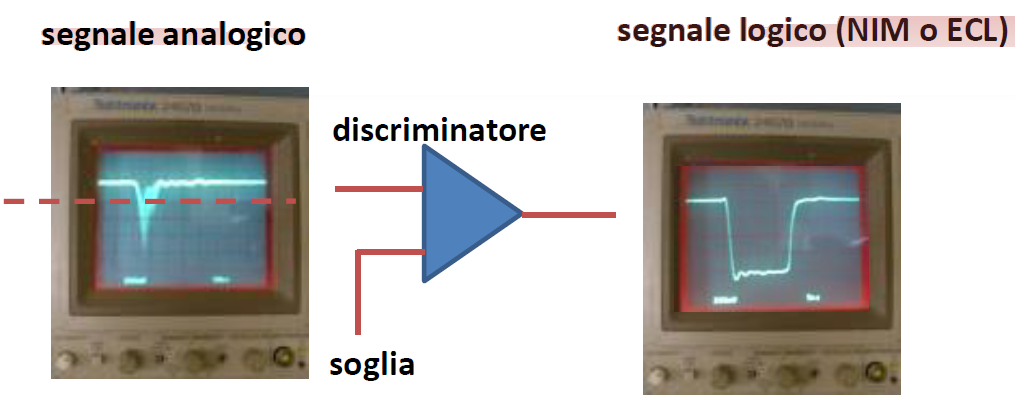
\includegraphics[width=0.8\textwidth]{immagini/segnale_discriminatore.png}
\end{figure}

Nel caso dei discriminatori, quindi, abbiamo in ingresso un segnale analogico come quello che vediamo visualizzato all'oscilloscopio nella figura sopra, decidiamo una soglia al di sotto della quale il segnale non viene presso in considerazione e attraverso questo circuito di soglia e un formatore si ottiene in uscita un segnale logico con un determinato standard.

Un discriminatore permette ad esempio di non prendere in considerazione nel sistema di acquisizione eventi in cui l'ampiezza del segnale è al di sotto di un certo valore. Infatti potremmo avere degli eventi dovuti a del rumore elettronico che tipicamente hanno ampiezze molto piccole, allora possiamo utilizzare un circuito di discriminazione per scartare e quindi non considerare tutti i segnali al di sotto di un certo valore, perché magari sappiamo che quei segnali non sono di interesse fisico ma sono più legati a un rumore elettronico. Un discriminatore era presente ad esempio nell'esperienza dei $\gamma$, però non lo vedevamo perché era qualcosa che si impostava via software. L'unico modo per accorgersene era notare che lo spettro che acquisivamo nei primi canali era sempre vuoto, cioè partiva da un certo canale in poi, e il motivo è che c'era impostata una soglia al di sotto della quale non veniva misurato nulla.

\subsection{Trasmissione dei segnali}

Sebbene trasportare un segnale sembri qualcosa di apparentemente banale, in realtà non è così, perché il segnale potrebbe subire delle deformazioni nel trasporto o anche nell'ingresso verso un modulo elettronico, soprattutto se è di natura analogica (quindi se è un segnale di cui ci interessa conoscere l'ampiezza o altre informazioni), per cui è chiaro che non bisogna deteriorare la qualità delle informazioni contenute nel segnale.

Nel trasporto dei segnali incorriamo principalmente in due problemi:

\begin{enumerate}[leftmargin=0.6cm]
   \item Abbiamo detto che idealmente vorremmo avere bande passanti infinite, ma poi nei fatti siamo costretti a utilizzare delle bande passanti limitate;
   \item Abbiamo la necessità di trasportare dei segnali su distanze che possono essere anche decine di metri.
\end{enumerate}

\section{Cavi}
La trasmissione dei segnali da una parte del sistema elettronico all'altra viene realizzata attraverso dei cavi. Precisiamo che parliamo di cavi e non di fili, in quanto sono cose diverse: non sono semplici fili elettrici come quelli che abbiamo utilizzato in Arduino.

\subsection{Cavi coassiali}
Guardiamo la struttura di un classico cavo che viene adoperato per trasportare del segnale:
\begin{figure}[H]
   \centering
   
\includegraphics[width=0.8\textwidth]{immagini/cavi_coassiali.png}
\end{figure}
Andando dall'interno verso l'esterno abbiamo:
\begin{itemize}
   \item un conduttore interno che è il portante del segnale;
   \item un dielettrico di separazione tra segnale e massa;
   \item una maglia che è uno schermo di fili intrecciati che rappresenta la massa, quindi è un altro materiale conduttivo;
   \item una guaina di protezione di materiale plastico che racchiude il tutto.
\end{itemize}
La struttura appena vista è tipica di un cavo coassiale. In realtà ci sono cavi anche più complessi, però quelli che adoperiamo in laboratorio sono di questo tipo.

La presenza del dielettrico comporta il fatto che il segnale viaggi a una velocità $v<c$, per cui il cavo induce un ritardo. Tipicamente per i cavi che adoperiamo si parla di ritardi di 5 nanosecondi ogni metro. Questa informazione del ritardo è così importante che tante volte i cavi vengono classificati non per lunghezza, ma per ritardo. 
%Quindi se vi capiterà poi il laboratorio di far attenzione a questo aspetto, andate a guardare nei cavi l'estremità. L'estremità c'è riportato una piccola spesso, volete riportato una piccola etichetta dove è riportato il ritardo di quel cavo. E tipicamente se prendete un cavo da un metro vi ritrovate appunto stampato 5 nanosecondi. 
Tale caratteristica dei cavi può essere sfruttata per creare appositamente il ritardo. Infatti potremmo essere interessati ad avere una linea di ritardo, quindi a ritardare un segnale rispetto a un altro, e se il ritardo è piccolo lo possiamo ottenere mettendo semplicemente del cavo. Bisogna però ricordare che oltre al ritardo il cavo introduce anche un'attenuazione, quindi più è lungo il cavo più segnale si attenua, per cui se siamo interessati ad esempio al trasporto di un segnale logico e lo vogliamo ritardare, dato che del segnale logico ci interessa poco l'attenuazione (ci interessa soltanto il fatto che ci sia o non ci sia ma che diminuisca leggermente l'ampiezza non è un problema), allora in quel caso si potrebbero adoperare decine di metri di cavo per poter produrre il ritardo desiderato.

Ci sono tantissime tipologie di cavo disponibili sul mercato che hanno caratteristiche molto diverse l'uno dall'altro. Quando si deve scegliere un cavo, ne andiamo a vedere non solo le caratteristiche geometriche come il diametro o il tipo (ad esempio coassiale o triassiale), ma anche altre informazioni come il ritardo, la capacità, l'attenuazione ecc. che sono tutte informazioni che servono quando si deve progettare un apparato e un trasporto di segnale. Ad ogni modo, i più utilizzati sono quelli riportati nella seguente tabella:

\begin{table}[H]
   \centering
   \begin{tabular}{|c|c|c|c|}
      \hline
      &&&\\[-0.3cm]
      Tipo & Ritardo [ns/m] & Diametro [cm] & Capacità [pF/m]\\[0.2cm]
      \hline
      &&&\\[-0.3cm]
      RG 58 & 5.14 & 0.307 & 93.5\\[0.2cm]
      \hline
      &&&\\[-0.3cm]
      RG 174 & 5.14 & 0.152 & 98.4\\[0.2cm]
      \hline
   \end{tabular}
\end{table}

l'RG 174 è la tipologia di cavo che abbiamo adoperato in laboratorio. Si tratta di un cavo abbastanza sottile avente un'impedenza di 50 $\Omega$, valore che è rilevante per quanto riguarda l'adattare il segnale in ingresso ai diversi apparati elettronici.

\subsection{Riflessione di un cavo}
Quando il segnale viaggia in un cavo ed entra in un modulo elettronico, ci dobbiamo assicurare che le impedenze del cavo e del modulo siano ben adattate, perché quello che potrebbe succedere è una parziale riflessione del segnale, che chiaramente è un effetto indesiderato perché potrebbe comportare delle distorsioni del segnale. L'effetto di questo adattamento dell'impedenza si può valutare mediante il coefficiente di riflessione del segnale, il quale è dato da
\begin{equation*}
   \rho=\frac{Z - Z_0}{Z + Z_0}
\end{equation*}
dove $Z_0$ è l'impedenza del cavo e $Z$ quella del carico esterno\footnote{Si intende qualsiasi altra strumentazione a cui viene collegato il cavo.}.

Distinguiamo due casi particolari:

\begin{itemize}[leftmargin=0.5cm]
   \item Se le impedenze sono uguali, cioè se $Z=Z_0$, ci troviamo nel caso ottimale in quanto $\rho=0$, cioè non c'è riflessione;
   \item Se invece l'impedenza esterna fosse nulla ($Z=0$), cioè se ci fosse un cortocircuito, avremmo che $\rho=-1$ e ci troveremmo nella condizione opposta estrema, in cui si ha una riflessione uguale ed opposta del segnale.
\end{itemize}
Appare dunque chiaro come, quando si deve trasportare un segnale, non bisogna tenere in conto soltanto il tipo di cavo con le sue caratteristiche, ma anche l'adattamento al carico esterno. In definitiva, in generale è necessario “terminare” un cavo coassiale con la sua resistenza caratteristica per evitare distorsioni nel segnale. Lo standard NIM parzialmente risolve questo problema, poiché la larga maggioranza dei moduli viene prodotta con impedenze di ingresso ed uscita pari a 50 $\Omega$. In alcuni casi ciò non è possibile, come ad esempio con un oscilloscopio. In questi casi la terminazione può essere realizzata utilizzando una resistenza (verso massa) esterna.

\subsection{Scelta del cavo}
Oltre che in base alla lunghezza del cavo, l'attenuazione cambia a seconda della frequenza, per cui quando scegliamo un cavo dobbiamo sapere qual è l'attenuazione alle frequenze tipiche dei segnali di nostro interesse.

Per calcolare l'attenuazione a un esatto valore di frequenza si possono utilizzare i cosiddetti nomogrammi, grafici in cui vengono riportate tre grandezze sulle loro scale. Conoscendo due grandezze, possiamo ricavare la terza attraverso un nomogramma unendo i due valori e andando a vedere l'intercetta nella terza scala.

In alternativa è possibile calcolare l'attenuazione totale del cavo mediante l'espressione
\begin{equation*}
   ALL=RL \cdot \sqrt{\frac{\textit{FA}}{\textit{FR}}}
   \qq{con}
   RL=\frac{R \cdot L}{100}
\end{equation*}
dove
\begin{itemize}[leftmargin=0.5cm]
   \item $R$ è il valore conosciuto della perdita a una data frequenza (dB/100 m o dB/100 ft);
   \item $L$ è la lunghezza del cavo (m o ft);
   \item $\textit{FR}$ è la frequenza alla quale è data la perdita (MHz);
   \item $\textit{FA}$ è la frequenza di lavoro alla quale si vuole calcolare la perdita (MHz);
   \item $ALL$ è la perdita totale del cavo a lunghezza $L$ e frequenza $\textit{FA}$.
\end{itemize}

\subsection{I connettori}
Alle estremità, i cavi hanno necessariamente un connettore. Ci sono svariati tipi di connettori, i quali possono essere pensati in maniera specifica per i segnali come ad esempio i connettori BNC o i connettori LEMO per i cavi a 50 $\Omega$ oppure dei connettori pensati per le alte tensioni come gli SHV e gli MHV. Ci sono anche diverse tipologie di connettori: maschi, femmine, a "T" a "I" ecc.

\begin{esempio}[Il connettore BNC]
   \begin{minipage}{0.39\textwidth}
      \begin{figure}[H]
         \centering
         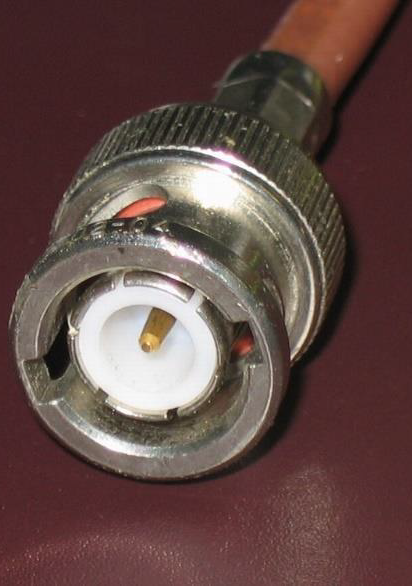
\includegraphics[width=0.9\textwidth]{immagini/connettore_BNC.png}
      \end{figure}
   \end{minipage}
   \begin{minipage}{0.6\textwidth}
      \vspace{0.6cm}In figura possiamo vedere un connettore BNC, che in laboratorio viene usato come connettore che mettiamo in ingresso all'oscilloscopio. \E composto da diverse parti: ha un pin centrale, l'isolante e un ground esterno e non è neanche facile assemblarlo, in quanto bisogna avere degli attrezzi specifici per assemblare questo tipo di connettori.\\
      Possono esserci diverse tipologie dello stesso connettore, ad esempio potremmo completare il BNC con una "T" per suddividere il segnale e quindi crearne una sorta di copia, anche se non è una copia esatta perché il segnale si divide, quindi se il segnale in ingresso ha una certa ampiezza in uscita dalle due estremità della "T" avremo un segnale che avrà un'ampiezza che è la metà.
   \end{minipage}
\end{esempio}
Ribadiamo che tutto ciò che si introduce per trasportare i segnali, se non ottimizzato, può creare delle distorsioni, che possono manifestarsi tramite gli effetti che abbiamo visto in precedenza di overshoot, undershoot, ringing e tilt.

\section{Come visualizzare i segnali: l'oscilloscopio}

Parliamo adesso della visualizzazione dei segnali. Il modo più semplice per visualizzare un segnale che viaggia attraverso un cavo è quello di inviarlo ad un oscilloscopio. Quest'ultimo lo possiamo banalmente immaginare come se fosse un voltmetro, quindi uno strumento che misura una differenza di potenziale, e che la rappresenta in un grafico in funzione del tempo, per cui quello che si visualizza nel monitor dell'oscilloscopio è il tempo sull'asse orizzontale e la tensione sull'asse verticale.

La principale distinzione per gli oscilloscopi è tra analogici e digitali. Un esempio di oscilloscopio analogico lo abbiamo visto nel corso di Laboratorio di Fisica II, il quale aveva il monitor fluorescente, mentre quello visto nelle esperienze di questo corso di laboratorio è un esempio di oscilloscopio digitale.

\subsection{Oscilloscopio analogico}
In figura possiamo vedere lo schema di base di un oscilloscopio analogico:
\begin{figure}[H]
   \centering
   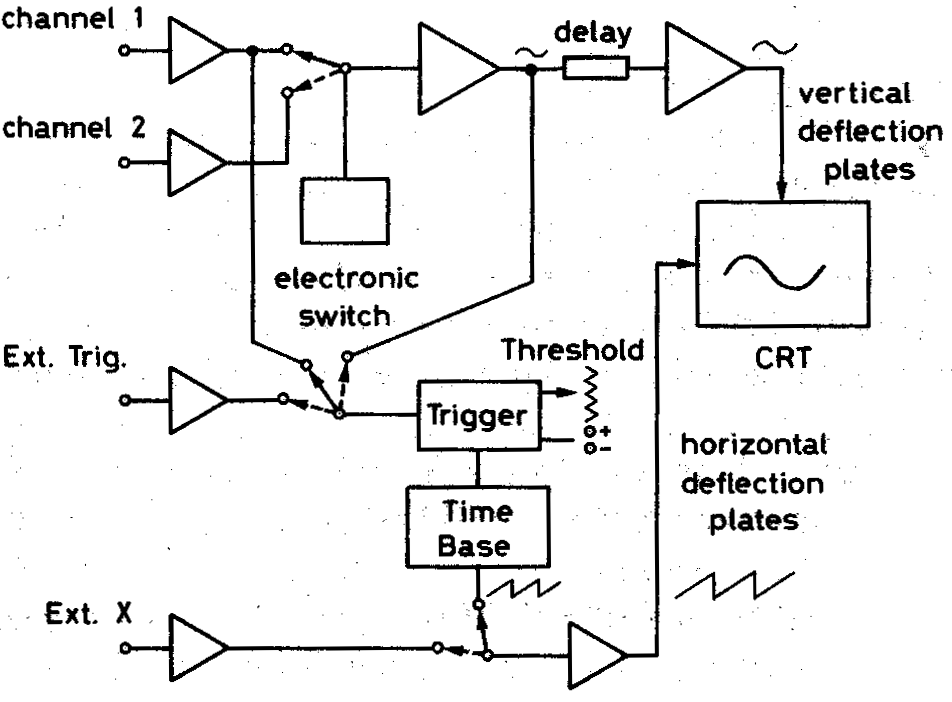
\includegraphics[width=0.6\textwidth]{immagini/schema_oscilloscopio_analogico.png}
\end{figure}
Vediamo innanzitutto che potremmo avere più ingressi (channel 1 e channel 2), quindi tale strumento ci permette di visualizzare simultaneamente più segnali che avranno la scala temporale in comune, mentre la scala verticale si può ottimizzare singolarmente per ogni segnale. Ciò che però è più importante ricordare sullo schema di funzionamento di un oscilloscopio analogico è il fatto che la traccia che viene visualizzata sul monitor viene prodotta attraverso un fascio di elettroni che viene fatto deviare utilizzando delle placchette orizzontali e placchette verticali a cui si applicano delle differenze di potenziale opportune, in particolare sulle placche orizzontali, che determinano il movimento orizzontale del fascio, si applica una tensione a dente di sega la quale fa sì che il fascio viaggi lungo l'asse orizzontale per poi improvvisamente tornare indietro ciclicamente, mentre sulle placche verticali si applica la differenza di potenziale che corrisponde al segnale da visualizzare, quindi il fascio verrà deviato in base al valore di tensione che sta arrivando in ingresso. Il risultato finale è una traccia visibile sul monitor dell'oscilloscopio.

\subsection{Banda passante}
Anche l'oscilloscopio ha una sua banda passante, quindi anche in questo caso dobbiamo capire l'effetto che potrebbe avere nella visualizzazione del segnale in ingresso per fare in modo che l'oscilloscopio rappresenti il segnale in modo corretto, in particolare per quel che riguarda il tempo di salita dei segnali. 

Supponiamo di inviare un segnale avente un tempo di salita che indichiamo con $t_{\rm rise}$. Quello che in realtà visualizziamo all'oscilloscopio sarà un tempo $t_{\rm meas}$ che è dato dalla somma in quadratura del tempo effettivo di salita del segnale più un tempo $t_{\rm osc}$ dettato dalle caratteristiche dell'oscilloscopio:
\begin{equation*}
   t_{\rm meas}=\sqrt{ t_{\rm rise}^2 + t_{\rm osc}^2 }
\end{equation*}
Questo tempo caratteristico dell'oscilloscopio si valuta utilizzando la seguente formula approssimata:
\begin{equation*}
   t_{\rm osc}=\frac{350}{f_{\rm 3 \, dB}[\rm MHz]}
\end{equation*}
dove $f_{\rm 3 \, dB}$ è la banda passante espressa in MHz. Quindi conoscendo la banda passante dell'oscilloscopio possiamo valutare a quanto ammonta il contributo dovuto all'oscilloscopio. \E chiaro che, se l'oscilloscopio è di buona qualità, tale contributo diventa abbastanza trascurabile perché più grande è la banda passante più questo valore è piccolo.

\subsection{Stadio di input}

Come ogni buon voltmetro, l'oscilloscopio ha un'alta impedenza di ingresso, tipicamente $1 \rm \; M\Omega$, in parallelo con una capacità di qualche decina di pF. Tuttavia quando inviamo un segnale con un cavo che solitamente ha un'impedenza intorno a 50 ohm conviene adattare le impedenze del cavo e del carico, per cui all'interno dell'oscilloscopio è possibile possibile modificare l'impedenza, in modo da terminare correttamente il cavo che trasporta il segnale.

Lo stadio di ingresso\footnote{Lo stadio di ingresso di un oscilloscopio è la parte iniziale del circuito dove viene applicato il segnale da misurare.} può essere in diverse modalità: può essere:
\begin{itemize}[leftmargin=0.5cm]
   \item DC, cioè accoppiato in continua, che è la modalità normale di funzionamento:
   \item AC, cioè viene filtrata la componente in continua;
   \item GND, cioè l'ingresso è posizionato al ground.
\end{itemize}

\subsection{Trigger}
Per trigger si intende una condizione che fa partire l'acquisizione di un evento o, nel caso particolare dell'oscilloscopio, la visualizzazione del segnale. Infatti potremmo essere interessati a voler vedere soltanto alcuni segnali che hanno un certo valore e altri no perché magari non sono di nostro interesse; oppure potremmo avere a che fare con un sistema di acquisizione che acquisisce dati e decidere di acquisire dati solo quando si verifica una determinata condizione, e entrambi i casi è necessario un sistema di trigger. Un esempio di trigger lo abbiamo usato nell'esperienza di laboratorio in cui si misura l'energia dei $\gamma$ emessi da una sorgente, dove si poteva decidere di mettere la condizione di misurare eventi, dunque segnali, aventi ampiezza superiore a un certo valore. Ciò costituisce un trigger perché si impone che l'acquisizione del dato avvenga quando tale condizione è verificata.

\E chiaro che quando abbiamo a che fare con un oscilloscopio non parliamo di vera e propria acquisizione perché non acquisiamo dati in termini di byte, bensì parliamo di visualizzazione. In particolare, per un oscilloscopio il trigger può essere

\begin{itemize}[leftmargin=0.5cm]
   \item interno se fa riferimento al segnale stesso che inviamo, quindi se poniamo una condizione sul segnale;
   \item esterno nel caso in cui l'acquisizione avviene quando riceviamo un segnale esterno, pertanto l'input e il segnale di trigger sono indipendenti.
\end{itemize}

\subsection{Oscilloscopio digitale vs oscilloscopio analogico}
Dato che oscilloscopio analogico e digitale hanno funzionalità analoghe, vediamo di fare un confronto tra le tue tipologie. 

La differenza principale è che nell'oscilloscopio digitale il segnale viene acquisito, quindi all'interno c'è un ADC che va a campionare il segnale in un certo numero di punti e lo rappresenta poi nel grafico come se fosse un segnale per punti, ed è tanto più fedele quanto più è grande il numero di punti che utilizza per rappresentare una forma d'onda, che è ciò che chiamiamo frequenza di campionamento.

Vediamo adesso di confrontarli in termini di prestazioni.

Partiamo dall'accuratezza, cioè quanto bene il segnale viene riprodotto:
\begin{itemize}[leftmargin=0.5cm]
   \item Nel caso dell'oscilloscopio analogico l'accuratezza dipende esclusivamente dalla banda passante;
   \item Nel caso dell'oscilloscopio digitale essa dipende dalla banda passante ma anche dalla frequenza di campionamento.
\end{itemize}
Abbiamo una differenza anche per quanto riguarda la sovrapposizione delle forme d'onda. Noi in laboratorio abbiamo utilizzato l'oscilloscopio per acquisire un solo segnale per volta, dunque non vedevamo forme d'onda sovrapposte, però in generale si potrebbe essere interessati a vedere delle forme d'onda sovrapposte per capire se ad esempio ci sono delle ampiezze più frequenti (il che appare all'oscilloscopio, dato che tanti segnali che si sovrappongono l'un l'altro, come delle zone più dense attorno alle ampiezze che si presentano con maggiore frequenza). Questa modalità è presente in entrambi gli oscilloscopi, però si basa su principi diversi:
\begin{itemize}[leftmargin=0.5cm]
   \item In quello analogico si sfrutta la permanenza della traccia nello schermo, quindi la "memoria" del fosforo;
   \item In quello digitale è dettata da un'operazione software, che dipende anche dalla capacità dell'oscilloscopio di memorizzare più forme d'onda e poterle rappresentare simultaneamente nello schermo.
\end{itemize}
All'inizio i primissimi modelli di oscilloscopi digitali non riuscivano a riprodurre bene questa modalità, ma oggigiorno sono competitivi tanto quanto quelli analogici.

Una differenza importante riguarda il trigger:
\begin{itemize}[leftmargin=0.5cm]
   \item Nel caso dell'oscilloscopio analogico la condizione di trigger si può imporre soltanto sull'ampiezza del segnale;
   \item In quello digitale invece normalmente è possibile adoperare trigger più complessi, che possono derivare anche da combinazioni logiche di segnali
\end{itemize}
Per capire la differenza supponiamo di avere un oscilloscopio digitale con 4 ingressi e di mandare a ciascun ingresso dei segnali in input. Supponiamo inoltre di essere interessati a vedere la forma d'onda soltanto quando abbiamo la coincidenza\footnote{Per coincidenza si intende quando due o più segnali arrivano simultaneamente.} tra tutti e quattro i segnali. Utilizzando un oscilloscopio digitale ciò si può fare da un punto di vista software, mentre per quello analogico dovremmo essere noi a realizzare la coincidenza in partenza, cioè produrre un segnale di coincidenza a parte con una modulistica dedicata per produrre un segnale di trigger che deve essere inviato all'oscilloscopio analogico per eventualmente acquisire i segnali.

Inoltre l'oscilloscopio digitale, proprio per il fatto che digitalizza l'informazione trasformandola in dati che possiamo salvare, ci permette di fare delle operazioni, quindi non solo lavorare sul trigger ma anche di fare degli analisi dei segnali in tempo in tempo (ad esempio si possono produrre degli spettri per i modelli più avanzati), quindi in generale ci sono delle funzionalità che quello analogico non possiede.

\comment{ci sono domande completo questa parte con questa idea che visto che abbiamo fatto appunto questi kit da utilizzare a casa con materiale abbastanza economico quindi il kit sul multimetro e il kit che utilizzano Arduino in realtà anche per quanto riguarda l'utilizzo di un uscizoscopio si può fare qualcosa a livello casalingue nel senso con costi molto bassi infatti sono stati immessi nel mercato degli uscizoscopi piccolini ovviamente magari a un solo canale che però hanno dei costi abbastanza contenuti dell'ordine di qualche decina di euro, venti, trenta euro e che permette di visualizzare segnali magari non segnali veloci come sono quelli che escono ad esempio da rivelatori come scintillatori o altro però segnali lenti come quelli che ad esempio avete gestito con i sensori di Arduino ecco se volete visualizzare qualcuno di questi segnali è possibile comprare uno di questi uscizoscopi tassalinghi che si presentano ad esempio come questo, questo viene dato in commercio, bisogna montare il pannello alla parte dell'elettronica però diciamo l'assemblage è molto semplice e vedete che prevede un solo ingresso con un connettore BNC che è uno dei connettori che abbiamo discusto la volta scorsa poi abbiamo un cavo con due puntali quindi questi puntali si adoperano proprio per andare a prelevare il segnale in alcuni punti ad esempio se avete a disposizione un sensore come quelli che avete operato per Arduino un'altra che alimenta il sensore potete provare a prelevare il segnale e visualizzarla all'uscilloscopio vedete sono dimensioni molto compatte decine di centimetri, il display è abbastanza piccolino però diciamo prevede la possibilità 

di fare un po' tutte le operazioni che si fanno tipicamente con oscilloscopio, qui sono riportate ad esempio le caratteristiche, possiamo vedere che la scala verticale varia da 10 mili volte 5 volte quindi è ottima la scala orizzontale è un po' più più vedete non potete andare al di sotto dei 10 microsecondi quindi non potete vedere segnali veloci se vi ricordate in laboratorio per visualizzare i segnali che venivano prodotti dallo scintillatore del fotonottibilitatore era necessario spandere la scala e renderla 20 nanosecondi per divisione, 10 non secondi per divisione quindi non siamo a questi livelli però per segnali lenti va più che bene tutte le modalità di trigger, auto, normal, singolo insomma tutto quello che fa un oscilloscopio professional ovviamente in scalari d'otta la larghezza della banda non è eccezionale ma d'altra parte ci lo aspettavamo, segnali veloci non li possiamo gestire perché la banda passante non ciò permette questo è un altro modello un po' più compatto ma anche più o meno meno stesso costo, monta addirittura il processo del primo, vedete qui lo schermo come è come appare, come permette di visualizzare i segnali più super rendervi i parteci di del fatto che esistono anche questi prodotti in commercio che sono veramente galini, veramente simpatici ci sono domande?}